 \documentclass[12pt]{article}
%%%%%%%%%%%%%%%%%%%%%%Paquetes
\usepackage[spanish]{babel}  
\usepackage{inputenc}%%%%%%%%%%%%ñ y acentos
\usepackage{tcolorbox}


\usepackage{fontspec}
\newfontface{\casio}{CASIOClassWiz}[
  Extension=.ttf,
]

\newfontface{\casiu}{CASIOMS01}[
  Extension=.ttf,
]


\newcommand{\casiosymbol}[1]{{\footnotesize\casio\symbol{#1}}}

\newcommand{\casiusymbol}[1]{{\footnotesize\casiu\symbol{#1}}}

\usepackage{fouriernc}


 \usepackage[papersize={188mm,210mm},left=3cm, right=3cm, top = 1cm, bottom = 1cm]{geometry}

\usepackage{latexsym,amsmath,amssymb,amsfonts}

\newcommand{\com}[1]{\textbf{\color{blue}{#1}}}

\pagestyle{empty}


\newenvironment{capitulo}{\begin{tcolorbox}[colback=blue!5!white,colframe=red!75!black]}{\end{tcolorbox}\bigskip}
\newenvironment{ejer}{\begin{tcolorbox}[center title, 
fonttitle=\sffamily\bfseries,colback=blue!5,colframe=orange]}{\end{tcolorbox}}
\newenvironment{funciones}{\begin{tcolorbox}[center title, title=Nuevas funciones, fonttitle=\sffamily\bfseries, colback=green!5!white,colframe=red!75!black]}{\end{tcolorbox}\bigskip}
\setlength{\parskip}{2mm}

\author{jltabara@gmail.com}

\title{Classwiz 991}

\date{}

\begin{document}

\begin{capitulo}

\vspace{-1cm}
\maketitle

\end{capitulo}

\vspace{-0.5 cm}

\thispagestyle{empty}

\tableofcontents
\newpage


\begin{capitulo}
 \addcontentsline{toc}{subsection}{Operaciones básicas}
\section*{Operaciones básicas}
\end{capitulo}



Para empezar a trabajar es conveniente resetear la calculadora. Debemos también estar en el \textbf{modo  Calcular}.

Si algún resultado nos da en forma de fracción y lo queremos en formato decimal, debemos pulsar la tecla \casiosymbol{110}:

\begin{ejer}

Realiza las siguientes operaciones:
\[
a)\,2+5, \qquad b)\,5-890 \qquad c)\,345 \times 34 \qquad d)\,(-3) \times 789
\]
\end{ejer}

\begin{ejer}

Opera y convierte el resultado en decimal:
\[
3.5 \times 4.3
\]

\end{ejer}

\begin{ejer}

A veces la operación no entra en pantalla:
\[
1+2+3+4+5+6+7+8+9+10+11
\]
\end{ejer}

\begin{ejer}

Las teclas del cursor nos permiten modificar operaciones:
\[
a)\, 3+40+5+6 \qquad b)\, 3+4+5+6
\]
\end{ejer}

\begin{ejer}

A veces las divisiones las trata como fracciones. Otras veces no:
\[
a)\, 345\div 24\qquad b)\, 34.67\div  4.2393
\]
\end{ejer}

\newpage
\begin{capitulo}
 \addcontentsline{toc}{subsection}{Potencias y operaciones combinadas}
\section*{Potencias y operaciones combinadas}
\end{capitulo}

Existen una tecla para calcular cuadrados, otra para calcular cubos y otra que sirve para elevar a cualquier potencia.

\begin{ejer}

Realiza las siguientes potencias:
\[
a)\, 2^2 \qquad b)\, 4^3 \qquad c)\, 24.5^{7} \qquad d) \,(-3)^4, \qquad e)\, 3.45^{2.46}
\]

\end{ejer}

En las operaciones combinadas lo primero que se realizan son los paréntesis, después las potencias, luego las divisiones y multiplicaciones y finalmente las sumas y restas. En definitiva, la calculadora sigue \textbf{la misma prioridad que se aplica en matemáticas}.

\begin{ejer}

Realiza las operaciones:
\[
a)\, 3+6\times 7 \qquad b)\, 36 \div 2^2 \qquad c)\, 
36 \div 6 \times 4
\]

\end{ejer}

\begin{ejer}

Realiza las siguientes operaciones combinadas:
\[
a) \, 4+(3-5)\times 67 +4^5 \qquad b)\, (2+4)^4-7+ 56\div 32
\]
\end{ejer}

En la calculadora no se pueden utilizar corchetes, pero si varios niveles de paréntesis.

\begin{ejer}
Realiza las siguientes operaciones:
\[
a)\,\left[2^5\left(4-3^2\right)\right] \div 22.5 \qquad b)\,
\left[34.78 \cdot \left(2.8-5\right)^2-3+7-89\right]^2
\]

\end{ejer}

\newpage

\begin{capitulo}
 \addcontentsline{toc}{subsection}{Divisibilidad}
\section*{Divisibilidad}
\end{capitulo}

Con la calculadora se pueden realizar ciertas operaciones que solamente tienen sentido si los números son enteros.


\bigskip

\begin{ejer}

Factoriza los siguientes números. Di cuales son primos:
\[
a)\, 360 \qquad \qquad b)\, 17 \qquad \qquad c)\, 5632563256
\]

\end{ejer}

\begin{ejer}

Realiza las operaciones y factoriza el resultado. Comprueba las reglas de las potencias:
\[
a)\, 5^3 \times 5^4 \qquad b)\, \frac{2^5}{2^2}\qquad c)\, \left(3^3\right)^4
\]

\end{ejer}

\begin{ejer}

Calcula el cociente y el resto de las divisiones y realiza la ``prueba'':
\[
a)\, 45 : 6 \qquad \qquad  b)\, 563256 :67
\]


\end{ejer}

\begin{ejer}

Calcula el MCM y el MCD de los siguientes números:
\[
a)\, 24\textrm{ y } 18 \qquad \qquad b)\, 455 \textrm{ y  } 900
\]

\end{ejer}


\newpage
\begin{capitulo}
 \addcontentsline{toc}{subsection}{Fracciones I}
\section*{Fracciones I}
\end{capitulo}

Los números decimales, si no son excesivamente grandes o pequeños, son transformados en fracciones por la calculadora.


\begin{ejer}
Escribe como fracciones, si es posible, los siguientes números decimales:
\[
a)\, 0.56 \qquad b)\, 0.5600 \qquad c)\, 0.512\qquad d)\, 45.987654
\]

\end{ejer}

La calculadora, si es posible, da siempre el resultado en forma de fracción simplificada.

\begin{ejer}

Simplifica las fracciones:
\[
a)\, \frac{20}{15} \qquad b)\, \frac{13}{5} \qquad c)\, \frac{2345}{8765} \qquad d)\, \frac{5\times 345}{3\times 345} 
\]

\end{ejer}

Aunque en España apenas se utiliza, las fracciones mayores que uno se pueden expresar en forma mixta: un número entero y la parte decimal en forma de fracción.

\begin{ejer} 

Expresa en forma mixta las fracciones:
\[
a)\, \frac{7}{5} \qquad b)\, \frac{456}{34}
\]

\end{ejer}

Un porcentaje no es más que una fracción de denominador 100. La calculadora en general simplifica dicho porcentaje.

\begin{ejer}

Escribe como fracciones los siguientes porcentajes:
\[
a)\, 75\% \qquad b)\, 40\% \qquad c)\, 34,6\%
\]
\end{ejer}





\newpage
\begin{capitulo}
 \addcontentsline{toc}{subsection}{Fracciones II}
\section*{Fracciones II}
\end{capitulo}

La calculadora realiza operaciones con fracciones y da el resultado simplificado. Si las fracciones son muy grandes entonces da directamente el resultado en formato decimal.

\begin{ejer} 

Realiza las operaciones:
\[
a)\,\frac{4}{3} + \frac{7}{3} \qquad b)\, \frac{13}{5}\times\frac{3}{8} \qquad c)\, \frac{6}{7} \div \frac{9}{13}
\]

\end{ejer}

También se pueden realizar operaciones combinadas. La jerarquía de operaciones es la habitual y se pueden emplear paréntesis.

\begin{ejer} 

Realiza las operaciones:
\[
 a)\,\left(\frac{4}{5}+ \left(\frac{7}{3} -\frac{4}{5}\right)^2\right) \times 5 - \left(\frac{3}{2}\right)^3
\qquad b)\,\frac{\frac{3}{4} \cdot 8}{\frac{4}{5} +\frac{2}{3}}
\]

\end{ejer}

Toda fracción es un número decimal exacto o bien es periódico. Para obtener el decimal asociado a una fracción escribimos la fracción y pulsamos la tecla \casiosymbol{110}. Para construir la fracción a partir del decimal, simplemente escribimos el decimal con ayuda de la tecla \casiosymbol{58}.

\begin{ejer}

Halla la fracción generatriz de:
\[
a)\,0.\wideparen{3} \qquad b)\, 45.\wideparen{39} \qquad c)\, 2.67\wideparen{21}\qquad d)\, 0.\wideparen{3} + \frac{2}{3}
\]

\end{ejer}

\newpage

\begin{capitulo}
 \addcontentsline{toc}{subsection}{Sustitución de variables}
\section*{Sustitución de variables}
\end{capitulo}

Dada una expresión algebraica, la calculadora  puede sustituir cada una de las letras por un valor y realizar las operaciones. Para ello debemos emplear la tecla \casiosymbol{114}.

Para empezar a realizar los cálculos de esta sección es conveniente resetear la calculadora para evitar que existan valores asignados a las variables. También podemos borrar únicamente la memoria.

\begin{ejer}

Calcular $x^3-6x+6$ para $x=5$.

\end{ejer}

\begin{ejer}

Calcular $5a^2+7b-\dfrac{3c}{4}$ para $a=5$, $b=6$, y $c=-2$

\end{ejer}

Los valores que escribamos en las letras quedan guardados y muchas veces no somos conscientes de ello. Con la tecla \textbf{Recall} podemos ver los valores asociados a cada letra. 



\begin{ejer}

Ver los valores almacenados en las variables con la tecla \textbf{Recall}.  Borra todas las variables. Vuelve a ver el contenido de las variables.



\end{ejer}

\newpage

\begin{capitulo}
 \addcontentsline{toc}{subsection}{Radicales I}
\section*{Radicales I}
\end{capitulo}

En la calculadora tenemos una tecla destinada a las raíces cuadradas, otra a las raíces cúbicas y otra más para realizar cualquier tipo de radical. Si el resultado no es el esperado, entonces debemos pulsar la tecla \casiosymbol{110} para convertir la raíz en decimal.



\begin{ejer}

Calcula las siguientes raíces exactas:
\[
a)\, \sqrt{16} \qquad b)\,\sqrt[3]{8} \qquad c) \, \sqrt[5]{32} \qquad  d)\, \sqrt[4]{3^8}
\]

\end{ejer}

\begin{ejer} 

Repetir lo anterior sabiendo que $\sqrt[n]{a}= a^{1/n}$.

\end{ejer}

Las potencias de exponente fraccionario y los radicales están íntimamente relacionados. Es más, utilizando la fórmula anterior es sencillo expresar cualquier radical como una potencia.

\begin{ejer} 

Calcula y relaciona las potencias con los radicales:
\[
a)\, 5^\frac{1}{2} \times 5^\frac{1}{2}\qquad b)\, 2^\frac{1}{3}\times 2^\frac{1}{3} \times 2^\frac{1}{3}
\]

\end{ejer}

\begin{ejer} 

Calcular como potencias y como radicales:
\[
a)\, 32^{3/4} \qquad  b)\, 23.78^{-2/5} 
\]

\end{ejer}

\begin{ejer} 

Realizar la siguiente operación combinada.
\[
\sqrt{5} +6 \times \sqrt[5]{9}
\]

\end{ejer}

\newpage

\begin{capitulo}
 \addcontentsline{toc}{subsection}{Radicales II}
\section*{Radicales II}
\end{capitulo}

Es bien conocido que se pueden realizar operaciones entre radicales de modo exacto y dar el resultado en forma de radical. La calculadora no realiza operaciones exactas con todos los tipos de radicales, pero en general, con los radicales cuadráticos si que realiza las operaciones en modo exacto.



\begin{ejer} 

Extraer factores de los radicales cuadráticos:
\[
a)\,\sqrt{8}  \qquad b) \,  \sqrt{243} \qquad c)\, \sqrt{\frac{8}{243}}
\]

\end{ejer}


\begin{ejer} 

Simplificar las operaciones con radicales:
\[
a)3\sqrt{20}- 7\sqrt{5} \qquad b)\, \sqrt{2}\sqrt{8} \qquad c)\, \sqrt{3}\sqrt{8}
\]

\end{ejer}

\begin{ejer} 

Racionalizar:
\[
a)\, \frac{3}{\sqrt{2}} \qquad b)\, \frac{2}{2+\sqrt{5}} \qquad c) \, \frac{6}{\sqrt{6}-\sqrt{2}}
\]

\end{ejer}



\newpage

\begin{capitulo}
 \addcontentsline{toc}{subsection}{Logaritmos}
\section*{Logaritmos}
\end{capitulo}

Los logaritmos en base 10 y los exponentes de potencias de base 10 están estrechamente relacionados. Se puede emplear la tecla $\log$ o bien la tecla general para todo tipo de logaritmos, poniendo la base igual a 10.

\begin{ejer}

Calcula los siguientes logaritmos en base 10.
\[
a)\, \log(10)\qquad b)\, \log(1000)\qquad c)\, \log\left(10^8\right) \qquad d)\, \log\left(10^{4,35}\right)
\]

\end{ejer}

Los logaritmos en base 2 están relacionados con los exponentes de potencias de base 2.

\begin{ejer}

Calcula los siguientes logaritmos en base 2.
\[
a)\, \log_2(2)\qquad b)\, \log_2(8)\qquad c)\, \log_2\left(2^8\right) \qquad d)\, \log_2\left(2^{4,35}\right)
\]

\end{ejer}

Los logaritmos en base 10 tienen una curiosa propiedad. El siguiente ejercicio te ayudará a desvelarla.

\begin{ejer}

Realiza los siguientes cálculos y observa el patrón:
\[
a)\, \log(3.2) \quad b)\, \log(32) \quad c)\, \log\left(3.2 \times 10^7\right) \quad d)\, \log\left(3.2 \times 10^{4.6}\right)
\]

\end{ejer}

Algo similar ocurre con los logaritmos en base 2.

\begin{ejer}

Realiza los siguientes cálculos y observa el patrón:
\[
a)\, \log_2(3.2) \quad b)\, \log_2\left(3.2\times 2^6\right) \quad c)\, \log_2\left(3.2 \times 2^{4.6}\right) 
\]

\end{ejer}


\newpage

\begin{capitulo}
 \addcontentsline{toc}{subsection}{Propiedades de los logaritmos}
\section*{Propiedades de los logaritmos}
\end{capitulo}

Las propiedades de los logaritmos nos permite calcular el logaritmo de un producto, de una división y de una potencia. Aunque esto no se puede demostrar con la calculadora, si se pueden comprobar en casos particulares.

\begin{ejer}

Realiza los siguientes cálculos y comprueba que son iguales:
\[
a)\log(45\times 32) \qquad b)\, \log(45) + \log(32)
\]
Comprueba que en otras bases se tiene también el mismo resultado en ambas operaciones.

\end{ejer}

Para la división y la potencia se tienen propiedades similares.

\begin{ejer}

Realiza los siguientes cálculos y comprueba que son iguales:
\[
a)\log_3\left(\frac{456}{34}\right) \qquad b)\, \log_3(456)-  \log_3(34)
\]

\end{ejer}

\begin{ejer}

Realiza los siguientes cálculos y comprueba que son iguales:
\[
a)\log_5(3.56^{4.1}) \qquad b)\, 4.1\times \log_5(3.56)
\]

\end{ejer}

La fórmula de cambio de base nos permite calcular logaritmos en cualquier base utilizando únicamente logaritmos decimales.

\begin{ejer}

Comprueba que son iguales:
\[
a)\log_{4.6}(5.78) \qquad b)\, \frac{\log(5.78)}{\log(4.6)}
\]

\end{ejer}

\newpage

\begin{capitulo}
 \addcontentsline{toc}{subsection}{Exponenciales y logaritmos}
\section*{Exponenciales y logaritmos}
\end{capitulo}

El número $e$ se puede definir de muchas formas, pero tal vez la más intuitiva nos dice que es igual a la expresión
\[
\left(1+\frac{1}{x}\right)^x
\]

\begin{ejer}

Calcula la expresión anterior para valores grandes de $x$ y comprueba que coincide con el número $e$

\end{ejer}

\begin{ejer}

Comprueba que $e^5$ es aproximadamente igual a la expresión
\[
\left(1+\frac{1}{x}\right)^{5x}
\]

\end{ejer}

\begin{ejer}

Realiza la operación:
\[
e^{4.61}+3\times e^{\frac{8}{3}}
\]

\end{ejer}



El logaritmo neperiano es justamente la función inversa de la función exponencial. Esto quiere decir que si primeramente elevamos $e$ a un número y al resultado le calculamos el logaritmo neperiano, el número no cambia.

\begin{ejer}

Realiza los siguientes cálculos:
\[
a)\, \ln\left(e^5\right) \qquad b)\, \ln\left(e^{34.5}\right) \qquad c)\, \ln\left(e^{-5.752}\right)
\]

\end{ejer}

De esto se deduce que la exponencial es la función inversa del logaritmo neperiano.

\begin{ejer}

Realiza las siguientes operaciones:
\[
a)\, e^{\ln(5)}\qquad b)\, e^{\ln(5.76)}
\]

\end{ejer}




\newpage

\begin{capitulo}
 \addcontentsline{toc}{subsection}{Grados y radianes}
\section*{Grados y radianes}
\end{capitulo}



Aunque cada vez se utilizan menos los grados minutos y segundos en la medida de los ángulos, puede ser conveniente saber transformar un ángulo dato en forma decimal a grados minutos y segundos.


\begin{ejer}

Transforma a notación sexadecimal (grados, minutos y segundos):
\[
a)\, 3.5 \qquad  b)\, 4.99 \qquad c) \, -8.923
\]
\end{ejer}

\begin{ejer}

Transforma de notación sexadecimal a decimal:
\[
a)\, 2^\mathrm{o} 45' 32'' \qquad b)\,56^\mathrm{o} 45''
\]

\end{ejer}

La calculadora también puede realizar operaciones básicas en notación sexadecimal. Si en algún caso nos entran dudas sobre la jerarquía de las operaciones siempre podremos utilizar paréntesis.

\begin{ejer}
Realiza las siguientes operaciones:
\[
a)\, 4^\text{o} 5' 34'' + 56^\text{o} 2'45'' \qquad b) \, 4\times(3^\text{o} 2')-2^\text{o} 0'57''
\]

\end{ejer}

La calculadora puede convertir grados en radianes y a la inversa. Si puede, la calculadora da los resultados en función de $\pi$.

Para cambiar a grados o radianes se utiliza el menú \casiusymbol{47}.

\begin{ejer}

Convierte en radianes (pon la calculadora en radianes):
\[
a)\, 180^\mathrm{o}\qquad b)\, 30^\mathrm{o}\qquad c)\, 45^\mathrm{o} \qquad d)\, 23.78^\mathrm{o}
\]

\end{ejer}

\begin{ejer}

Convierte en grados (pon la calculadora en grados):
\[
a)\, \frac{\pi}{3}\qquad b)\, \frac{5\pi}{3} \qquad c)\, \frac{13\pi}{6}
\]

\end{ejer}

\newpage

\begin{capitulo}
 \addcontentsline{toc}{subsection}{Trigonometría I}
\section*{Trigonometría I}
\end{capitulo}


Aunque lo mejor es trabajar en grados para hacer cálculos en grados, utilizando la tecla \casiosymbol{84} se puede añadir la unidad deseada.

\begin{ejer}

Trabajando en grados, calcula las siguientes razones trigonométricas (algunas deben calcularse en radianes):
\[
a)\sin(60^\mathrm{o}) \qquad b)\, \cos(78^\mathrm{o}) \qquad c)\, \sin\left(\frac{\pi}{3}\right)\qquad d)\,\tan\left(\frac{13\pi}{6}\right)
\]

\end{ejer}

Las funciones inversas  se llaman \texttt{Arcsin}, \texttt{Arccos} y \texttt{Arctan}. Debemos recordar que casi siempre existen dos soluciones para las funciones trigonométricas: una la proporciona la calculadora, la otra la debemos calcular nosotros.



\begin{ejer}

Calcula las dos soluciones y comprueba el resultado:
\[
\arcsin\left(\frac{\sqrt{2}}{2}\right)
\]

\end{ejer}

\begin{ejer}

Calcula las dos soluciones de:
\[
a)\, \arctan(\sqrt{3}) \qquad b)\,\mathrm{arccos}(0.345)
\]

\end{ejer}

\newpage

\begin{capitulo}
 \addcontentsline{toc}{subsection}{Trigonometría II}
\section*{Trigonometría II}
\end{capitulo}

La secante, la cosecante y la cotangente no tienen tecla en la calculadora, pero aún así su cálculo es muy sencillo.

\begin{ejer}

Calcula las siguientes razones trigonométricas:
\[
a)\, \sec(56) \qquad b)\, \mathrm{cosec}(34) \qquad  c)\, \mathrm{cotan}(123)
\]

\end{ejer}

Recordemos el teorema del coseno:
\[
a^2 = b^2+c^2-2bc\cos(\alpha)
\]
En esta calculadora es muy sencillo aplicar este teorema:

\begin{ejer}

En un triángulo dos lados miden 5 y 6 cm. El ángulo entre ellos es de $56^\mathrm{o}$. Calcula el lado que falta. Calcula también su área recordando la fórmula:
\[
A = \frac{1}{2} bc\mathrm{sen}(\alpha)
\]

\end{ejer}


\newpage

\begin{capitulo}
 \addcontentsline{toc}{subsection}{Funciones hiperbólicas}
\section*{Funciones hiperbólicas}
\end{capitulo}


Aunque no existen teclas para calcular funciones hiperbólicas, podemos acceder a ellas en la tecla \casiosymbol{84}.

\begin{ejer}

Calcula las razones hiperbólicas:
\[
a)\,\sinh(3) \qquad b)\, \tanh\left(\frac{8}{9}\right) \qquad c)\,\mathrm{arccosh}(4)
\]

\end{ejer}

Las funciones hiperbólicas se definen en función de las exponenciales. Por ejemplo:
\[
\sinh(x) = \frac{e^x-e^{-x}}{2}
\]

\begin{ejer}

Comprueba con alguno valores la verdad o falsedad de lo definición dada anteriormente de seno hiperbólico.

\end{ejer}

Como la gráfica de las funciones hiperbólicas no son muy conocidas, podemos esbozarlas con la calculadora y visualizarla con el código QR.

\begin{ejer}

Realiza una tabla de varios valores de la función $\sinh()$ y genera un código QR para visualizarla.

\end{ejer}

La relación fundamental de las funciones hiperbólicas es muy similar a la bien conocida de la trigonometría:
\[
\cosh^2(x)-\sinh^2(x)=1
\]

\begin{ejer}

Haz una tabla de valores para comprobar la validez de la fórmula anterior.
\end{ejer}



\newpage

\begin{capitulo}
 \addcontentsline{toc}{subsection}{Ecuaciones de segundo grado}
\section*{Ecuaciones de segundo grado}
\end{capitulo}

La calculadora puede resolver todo tipo de ecuaciones de segundo grado. Para ellos debemos estar en el modo \textbf{Ecuación/Func} y elegir dentro de él las ecuaciones polinómicas de segundo grado.

\begin{ejer}

Resuelve la ecuación:
\[
x^2-5x+6=0
\]

\end{ejer}

La curva asociada a toda ecuación de segundo grado es una parábola. La calculadora también nos da el vértice de dicha parábola.

Si una ecuación tiene una única solución, entonces el vértice debe estar situado en el eje $x$.

\begin{ejer}

Resuelve la ecuación y comprueba que el vértice está en el eje $x$:
\[
x^2+2x+1=0
\]

\end{ejer}


Entrando en la configuración de la calculadora, podemos decir si queremos las soluciones complejas o no.

\begin{ejer}

Resuelve con y sin soluciones complejas la ecuación:
\[
x^2+1=0
\]

\end{ejer}

Si generamos un código QR para una ecuación de segundo grado, además de la solución de la ecuación, nos da una gráfica de la parábola asociada.

\begin{ejer} 

Resuelve la ecuación y genera un código QR:
\[
-x^2+4x-13=0
\]

\end{ejer}

\newpage

\newpage

\begin{capitulo}
 \addcontentsline{toc}{subsection}{Ecuaciones de grado 3 y 4}
\section*{Ecuaciones de grado 3 y 4}
\end{capitulo}

De la misma forma que resuelve las de segundo grado puede resolver las de tercer y cuarto grado. También podemos o no incluir las soluciones complejas.

El conocimiento de las soluciones de las ecuaciones nos puede ser de gran ayuda en la factorización de polinomios.

\begin{ejer} 

Resolver las ecuaciones de tercer grado:

\bigskip

\begin{tabular}{l}
$a)\, x^3-6 x^2+11 x-6=0$\\
 \\
$b)\, x^3-3 x^2+x-3=0$\\
\\
$c)\, x^3-5 x^2+7 x-3=0$ \\
\\
$d)\, x^3-6 x^2+21 x-26=0$\\
\\
$e)\, 3.1x^3+5.23x+9=0$
\end{tabular}

\end{ejer}


\begin{ejer} 

Resuelve la ecuación de cuarto grado.

\bigskip
\begin{tabular}{l }
$a) \, x^4 - 6 x^3 + x^2 + 24 x - 20=0$ \\
\\
$b)\, x^4 - 3 x^3 + 4 x^2 - 6 x + 4=0$
\end{tabular}

\end{ejer}



\newpage

\begin{capitulo}
 \addcontentsline{toc}{subsection}{Sistemas de ecuaciones}
\section*{Sistemas de ecuaciones}
\end{capitulo}

La calculadora también resuelve sistemas de ecuaciones lineales con 2, 3 ó 4 ecuaciones. Para ello debemos entrar en el modo \textbf{Ecuación/Func} y elegir los sistemas lineales.


Si alguno de los sistemas tiene infinitas soluciones o no tiene ninguna (también llamados sistemas indeterminados o incompatibles) la calculadora nos informa, aunque en el caso de infinitas soluciones no nos proporciona la solución.

\begin{ejer}

Resuelve los siguientes sistemas de ecuaciones, comprobando que uno de ellos tiene solución única, otro infinitas soluciones o otro no tiene solución:

\bigskip

\begin{tabular}{l }

\bigskip
a) $\begin{cases}
3x + 4y &=11\\
2x - 7y & = -12
\end{cases}$\\

\bigskip
b) $\begin{cases}
3x + 4y &=34\\
6x + 8y & = 67
\end{cases}$\\

\bigskip
c) $\begin{cases}
3x + 4y &=34\\
6x + 8y & = 68
\end{cases}$\\

\end{tabular}

\end{ejer}

\begin{ejer} 


Resuelve los siguientes sistemas:

\begin{tabular}{l }

\bigskip

a) $\begin{cases}
3.7x + \sqrt{45}y &=1\\
\displaystyle 13x-67y& = \frac{3}{4}
\end{cases}$\\



b) $\begin{cases}
3x + 4y +5z  &=1\\
2x - 7y  +5z & = 2\\
-4 x +9y & = 3
\end{cases}$
\end{tabular}

\end{ejer}

\newpage


\begin{capitulo}
 \addcontentsline{toc}{subsection}{Números complejos I}
\section*{Números complejos I}
\end{capitulo}

Se pueden realizar todo tipo de cálculos con números complejos, ya sea en forma binómica o polar. Para realizar estos cálculos debemos estar en el modo \textbf{Complejo}. Si queremos que los resultados nos sean mostrados en forma binómica, debemos hacerlo en la configuración.

\begin{ejer}

Realiza las siguientes operaciones con complejos:
\[
a)\,  (3+5i) + (4+8i) \qquad b)\, (2-3i)\cdot (2-i)\qquad c)\, (3+i)\cdot 4_{20}
\]

\end{ejer}

\begin{ejer} 

Realiza las siguientes operaciones con complejos:
\[
a)\, \frac{2+7.6i}{2+8i}\qquad b)\, i^9\qquad c)\, \sqrt{-1}
\]

\end{ejer}

Un número complejo se representa como un vector en el plano. Por lo tanto tiene sentido calcular su módulo y su argumento. El módulo se calcula con la función \textbf{abs}. Para acceder al argumento debemos pulsar la tecla \casiosymbol{84}.

\begin{ejer}

Calcula el módulo y el argumento de los números:
\[
a)\, 3+4i \qquad b)\, 4i\qquad c) \, 6_{30}
\]

\end{ejer}




\newpage


\begin{capitulo}
 \addcontentsline{toc}{subsection}{Números complejos II}
\section*{Números complejos II}
\end{capitulo}

Si queremos que los resultados nos los proporcione en forma polar, debemos especificarlo en la configuración.

 
\begin{ejer}

Realiza las operaciones en forma polar:
\[
a)\, 2_{30} \cdot 5_{70}\qquad b)\, \left(3_{20}\right)^3 \qquad c)\, 2_{45} +(3+i)
\]

\end{ejer}


Estando en cualquier modo siempre podemos pasar de la forma binómica a la polar y viceversa. Las correspondientes funciones vuelven a estar en \casiosymbol{84}.



\begin{ejer}

Transforma en binómica los números:
\[
a)\,5_{30} \qquad b)\, 6_{56}
\]

\end{ejer}

\begin{ejer}

Transforma en polar los números:
\[
a)\, 4+i \qquad b)\, 6-7i
\]

\end{ejer}



En forma binómica el conjugado consiste en cambiar el signo a la parte imaginaria. En forma polar lo que cambia es el signo del argumento. La función para calcular argumentos está en \casiosymbol{84}.

\begin{ejer}

Calcula el conjugado de:
\[
a)\, 3+4i \qquad b)\, 4_{30}
\]

\end{ejer}

Además de estas funciones también podemos calcular la parte real e imaginaria en el menú \casiosymbol{84}.




\newpage

\begin{capitulo}
 \addcontentsline{toc}{subsection}{Combinatoria}
\section*{Combinatoria}
\end{capitulo}

La calculadora puede calcular factoriales y distintos números combinatorios. Para los números combinatorios se utiliza la tecla \textbf{nCr} y para el cálculo de variaciones la tecla \textbf{nPr}.


\begin{ejer}

Realiza las operaciones con factoriales (si es posible):
\[
a)\, 5! \qquad b)\, 70! \qquad c)\, \frac{10!}{3! \cdot  5!}
\]

\end{ejer}

\begin{ejer} 
Realiza las siguientes operaciones con variaciones sin repetición:
\[
a)\, \mathrm{V\,}_{23}^5\qquad b)\,\mathrm{V\,}_{10}^3  \qquad c)\, \frac{10!}{7!} \qquad d)\, \mathrm{V\,}_{12}^{12}
\]

\end{ejer}

\begin{ejer}

Realiza las siguientes operaciones con números combinatorios:
\[
a)\,\mathrm{C\,}_{10}^3\qquad b)\,\mathrm{C\,}_{10}^7\qquad c)\, \frac{10!}{7!\cdot 3!}\qquad  d)\,\mathrm{C\,}_{100}^1
\]

\end{ejer}


Otra cosa que puede hacer la calculadora es generar distintos tipos de números aleatorios. La tecla \textbf{Rnd\#} genera números aleatorios entre 0 y 1. La tecla \textbf{RanInt} genera números enteros.

\begin{ejer}

Genera distintos tipos de números aleatorios.

\end{ejer}


\newpage

\begin{capitulo}
 \addcontentsline{toc}{subsection}{Inecuaciones}
\section*{Inecuaciones}
\end{capitulo}

La calculadora resuelve inecuaciones polinómicas hasta grado 4. Debemos estar en el modo \textbf{Inecuación}.

\begin{ejer}

Resuelve la inecuación:
\[
x^2-5x+6 \geq 0
\]

\end{ejer}


Algunas inecuaciones pueden no tener solución o también que su solución sea el conjunto de todos los números reales.

\begin{ejer}

Resuelve las inecuaciones:
\[
a)\, x^2+1 >0 \qquad b)\, x^2+1 <0
\]


\end{ejer}


\begin{ejer}

Resuelve la inecuación (las soluciones de la ecuación son $2$, $3$ y $-5$):
\[
x^3 - 19 x + 30<0
\]


\end{ejer}

\begin{ejer}

Resuelve la inecuación:
\[
2x^4-3x^3-7x^2+5x+3 >0
\]

\end{ejer}




\newpage

\begin{capitulo}
 \addcontentsline{toc}{subsection}{Vectores I}
\section*{Vectores I}
\end{capitulo}

La calculadora puede trabajar con vectores de 2 y 3 dimensiones y realizar las operaciones básicas con ellos.  Para ello debemos estar en el modo \textbf{Vector}. 

\begin{ejer}

Dados los vectores $u=(3,2)$ y $v=(-6,1)$ calcula:
\[
 a) \, u+v  \qquad b)\,    u-v  \qquad c)\, 4u+7v 
 \]
 
\end{ejer}

Si nos hemos equivocado al introducir un vector, no es necesario teclearlo de nuevo. En lugar de eso podemos siempre que queramos editar los vectores y cambiar sus componentes.

\begin{ejer}

Edita el vector $v$ y cambia la coordenada $-6$ por $6$. Introduce un nuevo vector $w = (3,6)$ y realiza la operación:
\[
u+v+w
\]

\end{ejer}

El módulo de un vector lo calculamos con \textbf{Abs}.

\begin{ejer}

Calcula el módulo de $u$. Comprueba que su módulo es igual a la raíz cuadrada de sus componentes al cuadrado.

\end{ejer}

Para calcular el producto escalar debemos presionar \casiosymbol{84} e irnos a la segunda pantalla.

\begin{ejer}

Calcula:
\[
a)\, u \cdot v \qquad b)\, u\cdot u \qquad  c) \,|u|
\]

\end{ejer}

\begin{ejer}

Comprueba que los vectores $u=(4, 9)$ y $v=(-9,4)$ son perpendiculares.

\end{ejer}


\newpage

\begin{capitulo}
 \addcontentsline{toc}{subsection}{Vectores II}
\section*{Vectores II}
\end{capitulo}
 

Si estamos con vectores tridimensionales también se pueden calcular productos vectoriales. El producto vectorial se escribe con la tecla de multiplicación.

\begin{ejer}

Dados los vectores $u=(3,6,8)$ y $v=(1,8,-2)$, calcula los productos vectoriales:
\[
a)\, u \times v  \qquad b) \, v\times u \qquad c)\, u\times u
\]

\end{ejer}

Es un hecho conocido que el producto vectorial es perpendicular a cada uno de sus factores.

\begin{ejer} 

Comprueba que el siguiente resultado es nulo:
\[
(u\times v)\cdot u
\]

\end{ejer}

También es conocido que el área del paralelogramo que forman dos vectores es el módulo de su producto vectorial.

\begin{ejer}

Calcula el área del paralelogramo que forman los dos vectores.

\end{ejer}

Por último también se pueden calcular el ángulo que forman dos vectores y el vector unitario.

\begin{ejer} 

Calcula el vector unitario de $u$ y el ángulo que forman los vectores $u$ y $v$.

\end{ejer}

En las coordenadas de los vectores no es necesario introducir directamente números, también podemos escribir operaciones que la calculadora realiza y después asigna a la coordenada.

\begin{ejer}

Un vector tiene módulo 45 y forma un ángulo de 50 grados con el eje de las $x$. Introduce dicho vector.

\end{ejer}


\newpage

\begin{capitulo}
 \addcontentsline{toc}{subsection}{Matrices I}
\section*{Matrices I}
\end{capitulo}

Para trabajar con matrices debemos estar en el modo \textbf{Matriz}. Podemos introducir hasta 4 matrices distintas. Las matrices debe de ser de tamaño menor a $4\times 4$.

\begin{ejer}

Dadas las matrices:
\[
A=\begin{pmatrix}
2 & 3\\
5 & -1
\end{pmatrix} \qquad 
B =
\begin{pmatrix}
8 & -3\\
5 & 9
\end{pmatrix}
\]

calcula las combinaciones lineales:
\[
a)\, A+B\qquad  b)\, A-B\qquad c)\, 4A-7 B
\]

\end{ejer}

El producto de matrices se realiza con la tecla de multiplicar, o bien yuxtaponiendo ambas matrices.

\begin{ejer}

Calcula los siguientes productos:
\[
a)\,  A\cdot B \qquad   b)\, B \cdot A  \qquad c)\, A \cdot B \cdot A
\]

\end{ejer}


Las potencias de una matriz son multiplicaciones de la matriz por si misma. Por limitaciones técnicas,  la calculadora no realiza potencias superiores a 3.

\begin{ejer} 

Calcula las siguientes potencias:
\[
a)\, A^2 \qquad  b)\, A \cdot A\qquad  c)\, A^3 \qquad  d)\, A^4 
\]

\end{ejer}


\newpage

\begin{capitulo}
 \addcontentsline{toc}{subsection}{Matrices II}
\section*{Matrices II}
\end{capitulo}

Sin duda la potencia más interesante es la potencia $-1$ que nos permite calcular la inversa.

\begin{ejer}

Calcula:
\[
a)\, A^{-1} \qquad b)\, A^{-1} \cdot A
\]

\end{ejer}

Aunque la calculadora puede resolver sin problemas sistemas de ecuaciones lineales, también podemos utilizar el método de la matriz inversa.

\begin{ejer}

Dado el sistema de ecuaciones, resolver por la matriz inversa:

\[
\begin{cases}
2x-y+z &= 2\\
3x+y-2z & = 9\\
-x+2y+5z& = -5
\end{cases}
\]


\end{ejer}

Otras operaciones se realizan sobre una única matriz. Todos los comandos están en la segunda pantalla  de \casiosymbol{84}.


\begin{ejer}

Calcula el determinante de la matriz:
\[
A=\begin{pmatrix}
2 & 3 & 7\\
5 & -1 & 2 \\
3 & -7 & 1
\end{pmatrix}
\]

\end{ejer}

\begin{ejer}

Calcula la transpuesta de la matriz anterior.

\end{ejer}


\newpage

\begin{capitulo}
 \addcontentsline{toc}{subsection}{Matrices III}
\section*{Matrices III}
\end{capitulo}


La calculadora también es capaz de reducir por filas una matriz. Si la matriz representa un sistema de ecuaciones, ello equivale a realizar el método de Gauss. 




\begin{ejer}

Dado el sistema de ecuaciones, construir un sistema escalonado equivalente:

\[
\begin{cases}
2x-y+z &= 2\\
3x+y-2z & = 9\\
-x+2y+5z& = -5
\end{cases}
\]


\end{ejer}

También puede obtener la forma reducida, que equivale a realizar el algoritmo de Gauss-Jordan. De esta forma nos da la solución de modo inmediato.


\begin{ejer}

Resolver el sistema aplicando el algoritmo de Gauss-Jordan.


\end{ejer}



Con estos comandos se puede calcular el rango de matrices. El rango es el número de filas no nulas al reducir por filas la matriz.

\begin{ejer}

Calcula el rango de la matriz (la última fila es la suma de las dos primeras):
\[
\begin{pmatrix}
2 & 3 & 7\\
5 & -1 & 2 \\
7 & 2 & 9
\end{pmatrix}
\]



\end{ejer}



\newpage

\begin{capitulo}
 \addcontentsline{toc}{subsection}{Otras bases de numeración}
\section*{Otras bases de numeración}
\end{capitulo}



Además de la base decimal, la calculadora puede trabajar en base 2, 8 y 16. Para ello debemos entrar en el modo \textbf{Base n}.

\begin{ejer}

Convierte el número 456  a distintas bases de numeración. Lo mismo con $2AF_{16}$  y con 
 $10101011_2$.

\end{ejer}


Si nos situamos en una base la calculadora supone que todos los números que escribamos están en dicha base. Podemos realizar todo tipo de operaciones en dicha base.

\begin{ejer}

Realiza las operaciones en base binaria:
\[
a)\, 10101010 + 101011 \qquad b)\, 1001 \times 1111
\]

\end{ejer}




Además podemos hacer operaciones lógicas a nivel de bits. Lo ``lógico'' es trabajar en el modo binario para realizar estas operaciones.

\begin{ejer}

Calcula la tabla de verdad de la operación \textbf{and}.

\end{ejer}


\begin{ejer}

Realiza la operación:
\[
10101001 \textrm{ xor } 11110000
\]

\end{ejer}

\newpage

\begin{capitulo}
 \addcontentsline{toc}{subsection}{Resolución de ecuaciones}
\section*{Resolución de ecuaciones}
\end{capitulo}


En general las ecuaciones no se pueden resolver por métodos exactos. Por ello se suelen emplear métodos numéricos. Muchos de esos métodos parten de un número (llamado \textbf{semilla}) y se acercan progresivamente a una solución. Estos métodos no detectan cuantas soluciones tiene la ecuación y dependiendo de la semilla se acercan a una solución o a otra. 

\begin{ejer}


Resuelve la ecuación de primer grado:
\[
\frac{2(x-2)}{3} + 3x-7 = \frac{x}{7}
\]


\end{ejer}

\begin{ejer}

Resuelve la ecuación exponencial:
\[
3\cdot 4^x+9\cdot 2^x-30=0
\]

\end{ejer}

\begin{ejer}

Resuelve la ecuación trigonométrica con distintas semillas (tiene varias soluciones en el intervalo $(0,360)$):
\[
\cos(2x)+3\sin(x) =2
\]



\end{ejer}

\begin{ejer}

Resuelve la regla de tres directa:

\begin{center}
\begin{tabular}{c}
$3 \longrightarrow 7$ \\ 
$x \longrightarrow 89 $\\ 
\end{tabular} 
\end{center}


\end{ejer}

A veces la solución no se encuentra porque no existe.

\begin{ejer}

Ver que la siguiente ecuación no tiene solución:
\[
x^2+1=0
\]

\end{ejer}








\newpage

\begin{capitulo}
 \addcontentsline{toc}{subsection}{Estadística unidimensional}
\section*{Estadística unidimensional}
\end{capitulo}

Para realizar cálculos estadísticos en una variable debemos ir al modo \textbf{Estadística} y elegir \textbf{1-Variable}.

\begin{ejer}

Calcula los parámetros estadísticos de los datos:
\[
5, 7, 7, 8, 9, 10
\]

\end{ejer}

Por defecto la calculadora viene con la columna de  frecuencias desactivada. Para activarla debemos ir a \textbf{Configuración/Estadística}.

\begin{ejer}

Dada la tabla de frecuencias:
\begin{center}
\begin{tabular}{c|c}
x & f \\ \hline
3 & 4 \\
4 & 7 \\
6 & 5\\
7 & 5
\end{tabular}
\end{center}
calcula todos los parámetros estadísticos.

\end{ejer}

Si queremos seguir operando con los  resultados debemos acceder a cada uno de los parámetros estadísticos individualmente. Para ello debemos acceder a la segunda pantalla de \casiosymbol{84}.

\begin{ejer}

Calcula el coeficiente de variación:
\[
CV = \frac{\sigma}{\bar x}
\]

\end{ejer}

\begin{ejer}

Calcula el rango intercuartílico: $R_I=Q_3 - Q_1$.

\end{ejer}





\newpage

\begin{capitulo}
 \addcontentsline{toc}{subsection}{Estadística bidimensional}
\section*{Estadística bidimensional}
\end{capitulo}

La calculadora puede calcular varios parámetros estadísticos bidimensionales y hacer varios tipos de regresiones. Los parámetros estadísticos no dependen de la regresión que elijamos. 

Para realizar los cálculos vamos a realizar una regresión lineal. Debemos estar en el modo \textbf{Estadística/y=a+bx}.

\begin{ejer}

Calcula todos los parámetros estadísticos bidimensionales de la tabla:

\begin{center}
\begin{tabular}{c|c}
x & y \\ \hline
3 & 4 \\
4 & 5.2 \\
6 & 7.3\\
7 & 8
\end{tabular}
\end{center}

Calcular la covarianza. La fórmula es:
\[
\sigma_{xy} = \frac{\sum x_i \cdot y_i}{n} - \bar x \cdot \bar y
\]

\end{ejer}

\begin{ejer}

Calcula la recta de regresión de $y$ sobre $x$ y el coeficiente $r$.

\end{ejer}

\begin{ejer}


Estima el valor de $y$ cuando $x= 6.3$.

Estima el valor de $x$ cuando $y=6$.


\end{ejer}

\begin{ejer}

Calcula otros tipos de regresiones que no sean lineales.


\end{ejer}





\newpage

\begin{capitulo}
 \addcontentsline{toc}{subsection}{Distribución normal}
\section*{Distribución normal}
\end{capitulo}


La distribución normal depende de dos parámetros: $\mu$ y $\sigma$. La gráfica de la función para $\mu=0$ y $\sigma=1$ es:

\begin{center}
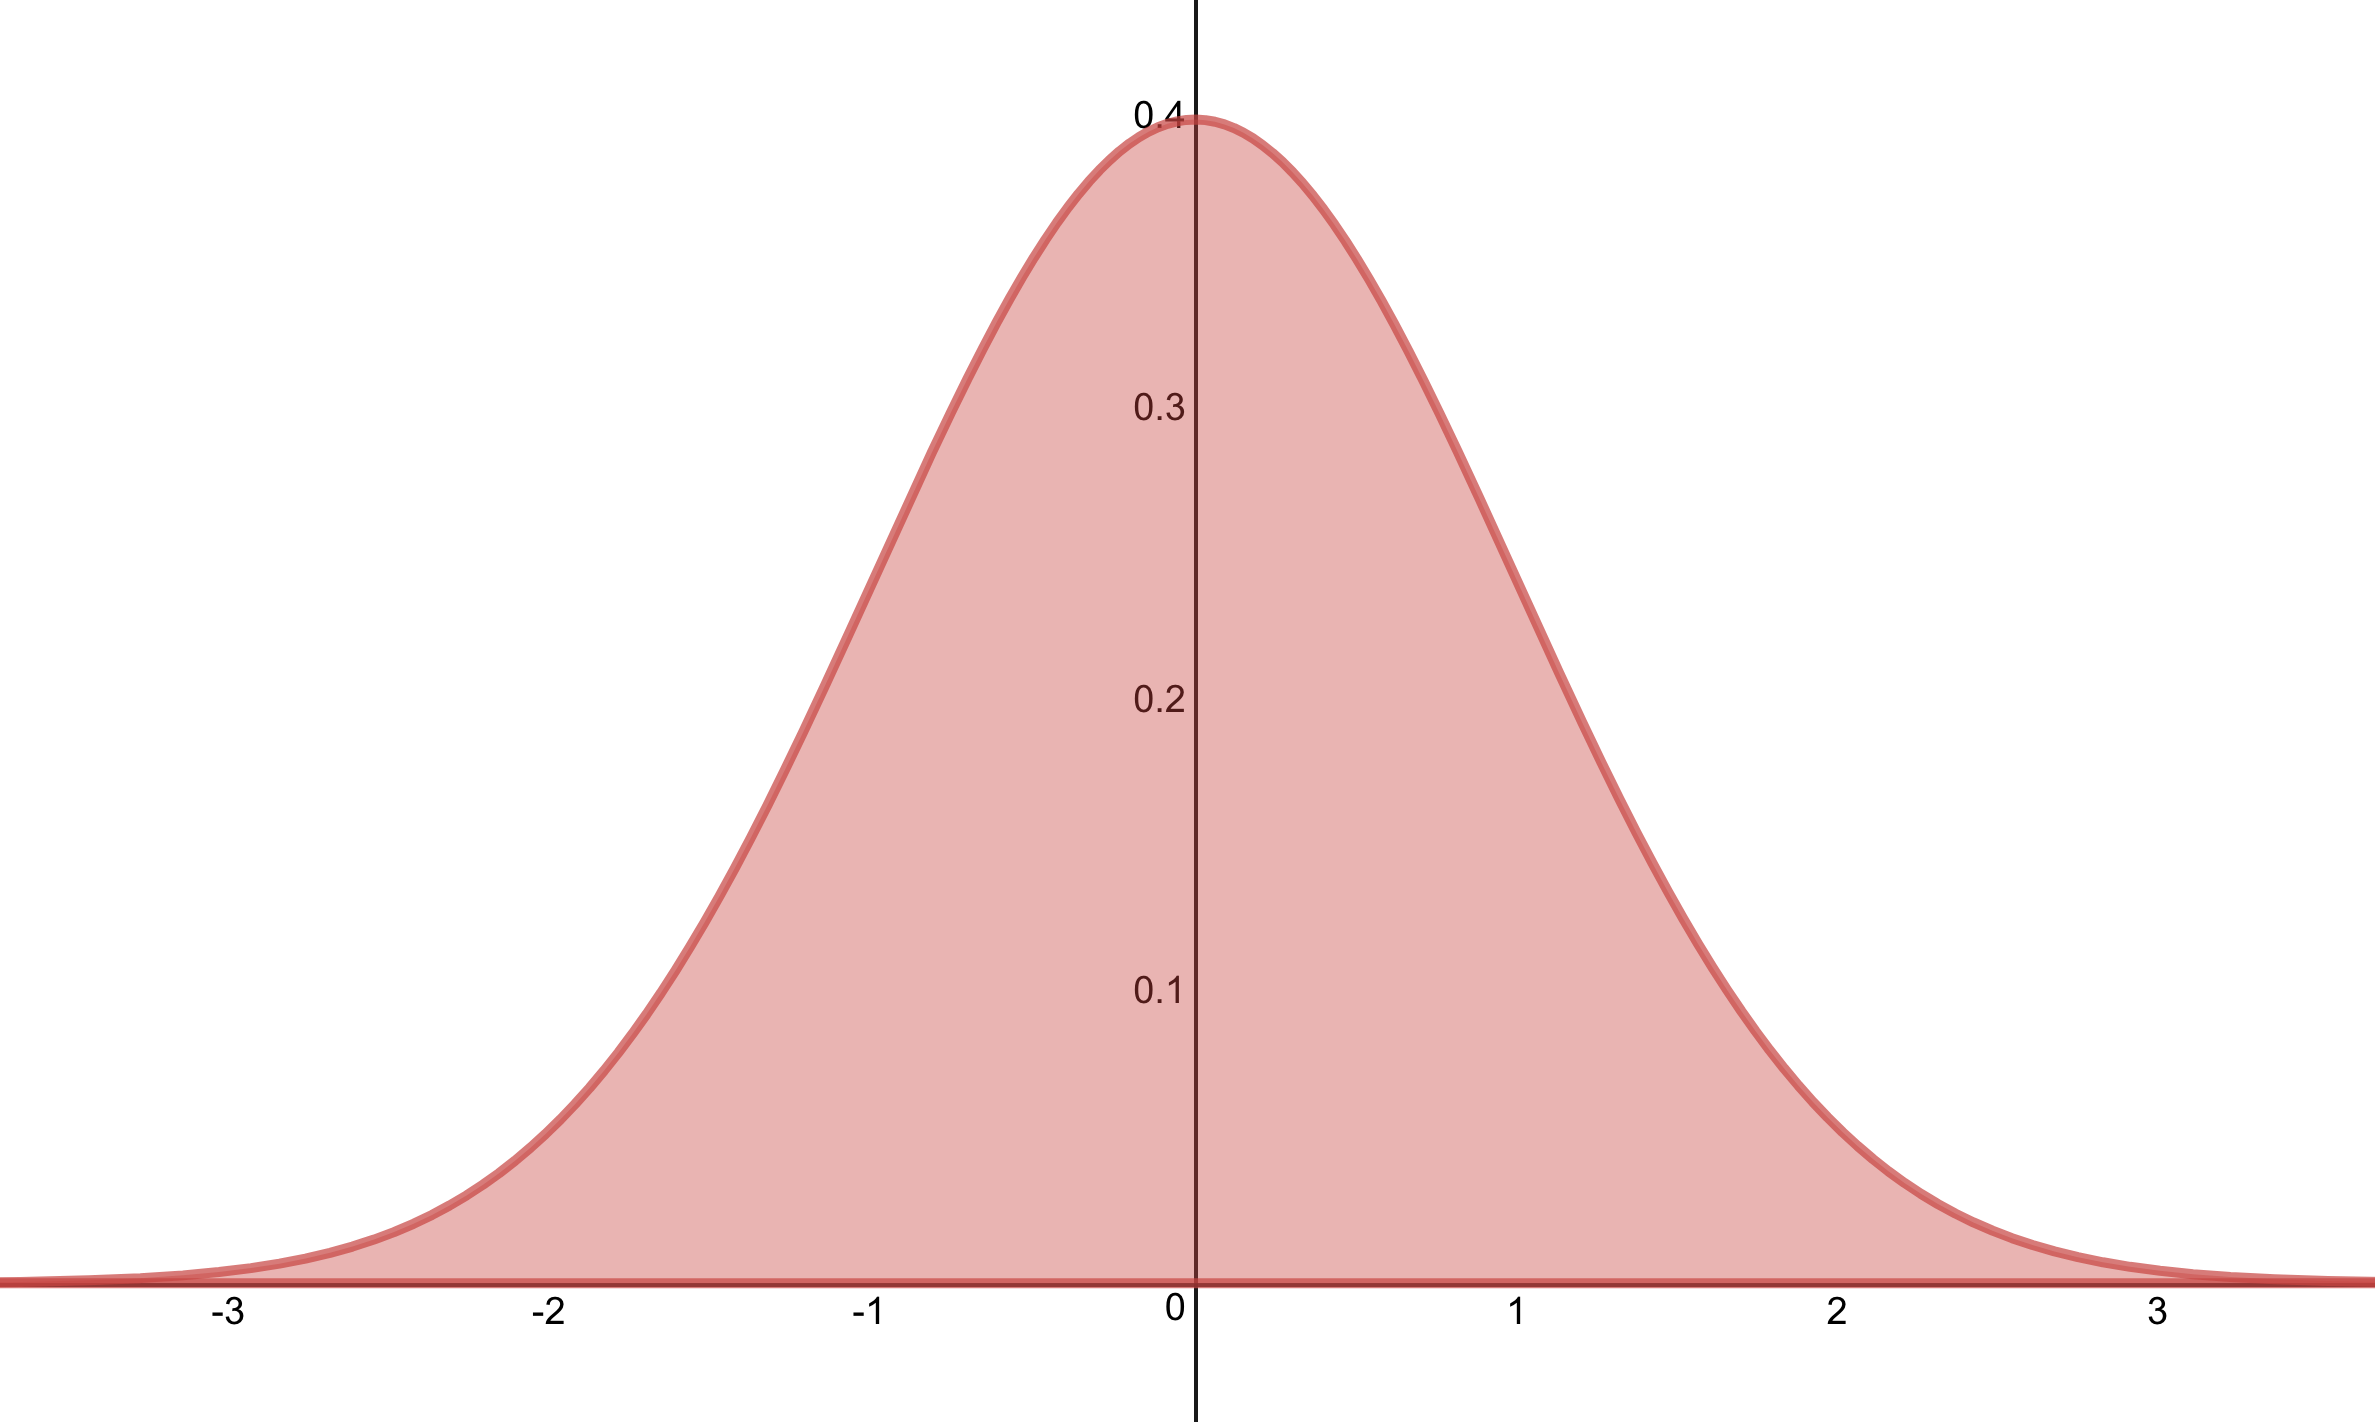
\includegraphics[width=7cm]{Normal.png} 
\end{center}

Entrando en el menú  \textbf{Distribución} y con la función \textbf{DP Normal} podemos calcular valores de dicha función.

\begin{ejer}

Calcula el valor de la función normal para distintos valores de $x$. Se pueden variar también los valores de la media y la desviación típica.


\end{ejer}

Con la orden \textbf{DP Normal}, que da acceso a la distribución acumulada, se pueden calcular distintas probabilidades. Como no podemos poner infinito, ponemos un valor lo suficientemente grande.

\begin{ejer}

Si $X \sim N(\mu=3, \sigma = 4)$ calcula:
\[
a)\,P(X<4)\qquad b)\, P(-3 < X< 6) \qquad c)\, P(X>2)
\]

\end{ejer}

Con la instrucción \textbf{Normal Inversa} calcular el número asociado a una cierta probabilidad.

\begin{ejer}

Si $X \sim N(\mu=3, \sigma = 4)$ calcula el valor $x$ que hace que:
\[
P(X \leq x) = 0.95
\]

\end{ejer}


\newpage

\begin{capitulo}
 \addcontentsline{toc}{subsection}{Distribución binomial}
\section*{Distribución binomial}
\end{capitulo}

La distribución binomial depende de dos parámetros, $n$, el número de intentos y $p$, la probabilidad de éxito.

En la figura se muestra la distribución para $n=20$ y $p=0.4$.

\begin{center}
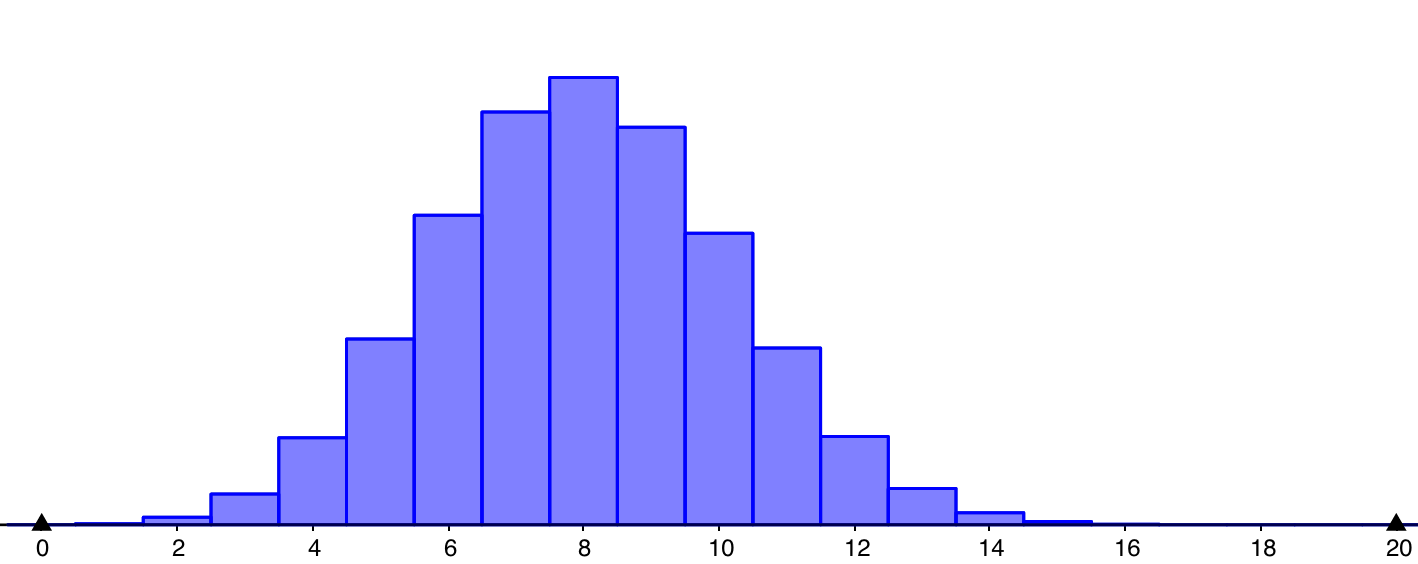
\includegraphics[width=7cm]{Binomial.png} 
\end{center}

Entrando en el menú  \textbf{Distribución} y con la función \textbf{DP Binomial} podemos calcular la altura de las barras.

\begin{ejer}

Si $X \sim Bin(n=20, p=0,4)$ calcula las probabilidades:
\[
a)\,P(X=4)\qquad b)\, P(X=8)\qquad c)\, P(X=20)
\]

\end{ejer}

Con la función acumulada \textbf{DA Binomial} podemos calcular la cola izquierda de la función. Debemos tener en cuenta que la distribución es discreta, para el cálculo de probabilidades donde aparezca un signo $<$.

\begin{ejer}

Si $X \sim Bin(n=20, p=0,4)$ calcula las probabilidades:
\[
a)\, P(X \leq 4) \qquad b)\,P(X \leq 20) \qquad c)\, P(X < 7)
\]

\end{ejer}


\newpage

\begin{capitulo}
 \addcontentsline{toc}{subsection}{Sumatorios}
\section*{Sumatorios}
\end{capitulo}



La suma de los primeros $n$ números naturales:
\[
\sum_{i=1}^n i = \frac{n(n+1)}{2}
\]

\begin{ejer}

Suma los 100 primeros números naturales.

\end{ejer}

La suma de los cuadrados de los números naturales:
\[
\sum_{i=1}^n i^2 = \frac{n(n+1)(2n+1)}{6}
\]

\begin{ejer}

Suma los cuadrados de los 100 primeros números naturales.

\end{ejer}

Una conocida serie que aproxima al número $e$ es:
\[
e = \sum_{i=0}^\infty \frac{1}{i!} 
\]


\begin{ejer}

Calcula distintas aproximaciones del número $e$.

\end{ejer}

\begin{ejer}

Suma las 40 primeras potencias de 2.

\end{ejer}


\begin{ejer}

Suma los 100 primeros números de la sucesión $a_n = 3n+6$.

\end{ejer}


\newpage

\begin{capitulo}
 \addcontentsline{toc}{subsection}{Opciones de configuración}
\section*{Opciones de configuración}
\end{capitulo}

Se puede configurar la calculadora para cambiar el modo de introducir y presentar resultados. 

\begin{ejer}

Efectua los siguentes cálculos en los cuatro modos de \textbf{Entrada/Salida} que presenta la calculadora:
\[
a)\, \frac{2}{5} \qquad \qquad b)\, \sin(45)
\]


\end{ejer}


También podemos indicarle con cuantos decimales nos presenta el resultado:

\begin{ejer}

Realiza los siguientes cálculos en las cuatro opciones de \textbf{Formato número}:
\[
a)\, \frac{2}{5} \qquad \qquad b)\, \sin(45)
\]


\end{ejer}

Los resultados los muestra en forma de fracción impropia, pero también podemos pedirle a la calculadora que lo muestre como número mixto.

\begin{ejer}

Cambiando la configuración de las fracciones, realiza:
\[
a)\, \frac{6}{5} \qquad \qquad b)\, \frac{45}{7}
\]


\end{ejer}

\begin{ejer}

Activa la fuente pequeña y realiza algunos cálculos.


\end{ejer}

\newpage

\begin{capitulo}
 \addcontentsline{toc}{subsection}{Integrales y derivadas}
\section*{Integrales y derivadas}
\end{capitulo}

La calculadora puede calcular integrales definidas por métodos numéricos. Para ello tenemos que introducir la función y los dos límites de integración.



\begin{ejer}

Calcula las integrales:\vspace{-3mm}
\[
a)\, \int_0^1 x\, dx \qquad b)\, \int_0^3 4x^2-3x\, dx  \qquad c)\,b)\, \int_0^3 4x^2-3x\, dx
\]

\end{ejer}

Es importante \textbf{trabajar siempre en radianes} cuando se realicen integrales y derivadas de funciones trigonométricas.

\begin{ejer}
Calcula la siguiente integral, en grados y radianes: \vspace{-3mm}
\[
 \int_{\frac{-\pi}{2}}^{\frac{\pi}{2}} \cos(x)\, dx
\] 

\end{ejer}

La integral de una función no siempre es el área bajo la curva.

\begin{ejer}

Calcula las siguientes integrales: \vspace{-3mm}
\[
a)\,\int_{-3}^3 x^3\, dx \qquad \int_{-3}|x^3|^3 \, dx
\]

\end{ejer}

También puede calcular derivadas en un punto de cualquier función, empleando también métodos numéricos.

\begin{ejer}

Calcula las derivadas:\vspace{-3mm}
\[
a)\, \frac{d}{dx}(x^3-3x)_{|x=2}\qquad  b)\, \frac{d}{dx}(x^3-3x+32)_{|x=2}\qquad \, \frac{d}{dx} \cos(x^2)_{|x=\pi}
\]

\end{ejer}

\begin{ejer}

Calcular la recta tangente a la curva $y=x^3-5x$ en el punto $x=2$.


\end{ejer}


\newpage

\begin{capitulo}
 \addcontentsline{toc}{subsection}{Estimación de límites}
\section*{Estimación de límites}
\end{capitulo}

\newpage

\begin{capitulo}
 \addcontentsline{toc}{subsection}{Conversiones}
\section*{Conversiones}
\end{capitulo}


\newpage

\begin{capitulo}
 \addcontentsline{toc}{subsection}{Miscelanea}
\section*{Miscelanea}
\end{capitulo}


Guarda valores en variables y recuperarlos

Calcular productorios

Calcular derivadas

Calcular integrales

Constantes integradas


\newpage

Introducir numero en notacion cientifica

Utilizar teorema del seno para resolver triangulos



Guardar en variables.




Comprobar seno al cuadrado mas coseano al cuadrado es 1

comprobar que tangente se igual a seno partido coseno.

hacer una tabla de la funcion seno en radianes.










\end{document}

